\documentclass[tikz]{standalone}
\usetikzlibrary{arrows, positioning}
\tikzset{
  treenode/.style = {align=center, inner sep=1pt, text centered,
    font=\sffamily},
  arn_b/.style = {treenode, circle, white, font=\sffamily\bfseries, draw=black,
    fill=black, text width=2.5em},% arbre rouge noir, noeud noir
  arn_r/.style = {treenode, circle, red, draw=red, 
    text width=2.5em, very thick}% arbre rouge noir, noeud rouge
}
\tikzstyle{every node}=[font=\Large]
\begin{document}
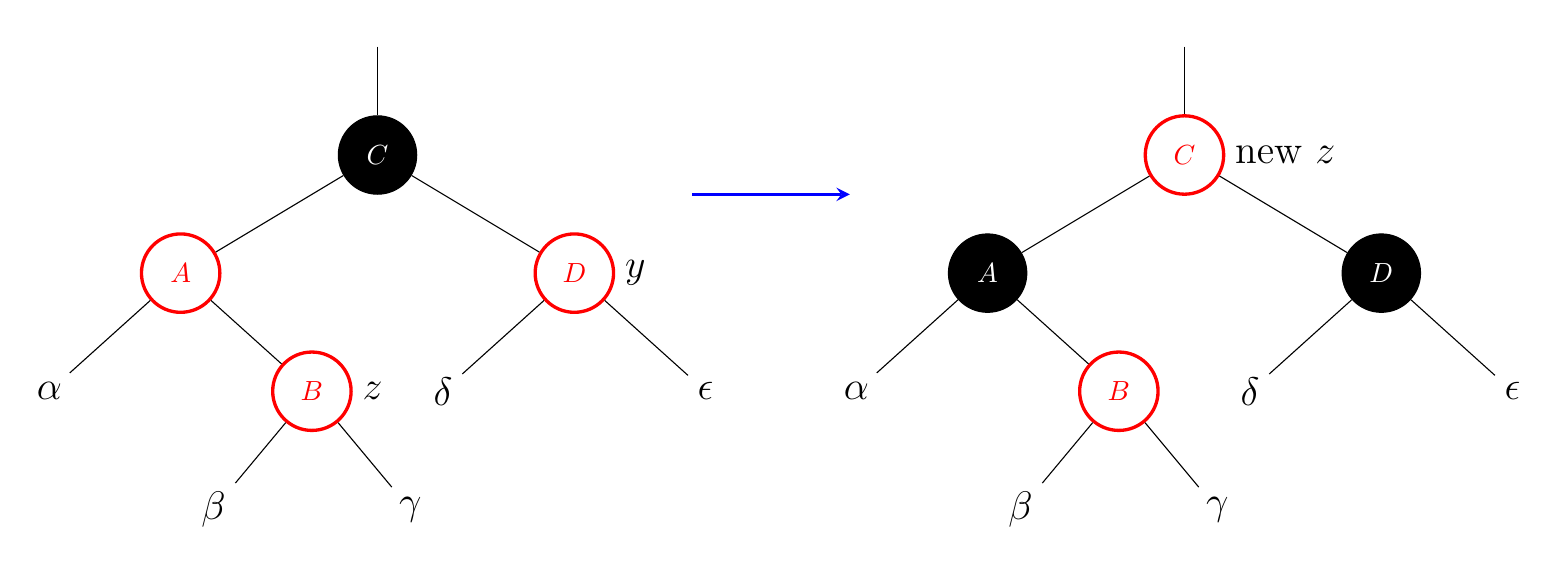
\begin{tikzpicture}[level/.style={sibling distance = 10cm/#1,
    level distance = 1.5cm}]
    \node (lefttree) {}
     child {node [arn_b] {$C$} 
            child {node [arn_r] {$A$}
            child {node {$\alpha$}}
            child {node (anb) [arn_r] {$B$}
                child {node {$\beta$}}
                child {node {$\gamma$}}
            }
        }
        child {node (and) [arn_r] {$D$}
        child {node {$\delta$}}
        child {node {$\epsilon$}}
        }
     }
    ;
    \node [right] at (anb.east) {$z$};
    \node [right] at (and.east) {$y$};

    \draw [-stealth, line width=0.4mm, draw=blue](4,-2) -- (6,-2)node[midway,above,shape=rectangle,draw=none]{};


    \node (righttree) [right=of lefttree, xshift=9cm] {}
    child {node (bcn) [arn_r] {$C$} 
           child {node [arn_b] {$A$}
           child {node {$\alpha$}}
           child {node  [arn_r] {$B$}
               child {node {$\beta$}}
               child {node {$\gamma$}}
           }
       }
       child {node [arn_b] {$D$}
       child {node {$\delta$}}
       child {node {$\epsilon$}}
       }
    }
   ;
    \node [right] at (bcn.east) {new $z$};
\end{tikzpicture}
\end{document}